\documentclass[1p]{elsarticle_modified}
%\bibliographystyle{elsarticle-num}

%\usepackage[colorlinks]{hyperref}
%\usepackage{abbrmath_seonhwa} %\Abb, \Ascr, \Acal ,\Abf, \Afrak
\usepackage{amsfonts}
\usepackage{amssymb}
\usepackage{amsmath}
\usepackage{amsthm}
\usepackage{scalefnt}
\usepackage{amsbsy}
\usepackage{kotex}
\usepackage{caption}
\usepackage{subfig}
\usepackage{color}
\usepackage{graphicx}
\usepackage{xcolor} %% white, black, red, green, blue, cyan, magenta, yellow
\usepackage{float}
\usepackage{setspace}
\usepackage{hyperref}

\usepackage{tikz}
\usetikzlibrary{arrows}

\usepackage{multirow}
\usepackage{array} % fixed length table
\usepackage{hhline}

%%%%%%%%%%%%%%%%%%%%%
\makeatletter
\renewcommand*\env@matrix[1][\arraystretch]{%
	\edef\arraystretch{#1}%
	\hskip -\arraycolsep
	\let\@ifnextchar\new@ifnextchar
	\array{*\c@MaxMatrixCols c}}
\makeatother %https://tex.stackexchange.com/questions/14071/how-can-i-increase-the-line-spacing-in-a-matrix
%%%%%%%%%%%%%%%

\usepackage[normalem]{ulem}

\newcommand{\msout}[1]{\ifmmode\text{\sout{\ensuremath{#1}}}\else\sout{#1}\fi}
%SOURCE: \msout is \stkout macro in https://tex.stackexchange.com/questions/20609/strikeout-in-math-mode

\newcommand{\cancel}[1]{
	\ifmmode
	{\color{red}\msout{#1}}
	\else
	{\color{red}\sout{#1}}
	\fi
}

\newcommand{\add}[1]{
	{\color{blue}\uwave{#1}}
}

\newcommand{\replace}[2]{
	\ifmmode
	{\color{red}\msout{#1}}{\color{blue}\uwave{#2}}
	\else
	{\color{red}\sout{#1}}{\color{blue}\uwave{#2}}
	\fi
}

\newcommand{\Sol}{\mathcal{S}} %segment
\newcommand{\D}{D} %diagram
\newcommand{\A}{\mathcal{A}} %arc


%%%%%%%%%%%%%%%%%%%%%%%%%%%%%5 test

\def\sl{\operatorname{\textup{SL}}(2,\Cbb)}
\def\psl{\operatorname{\textup{PSL}}(2,\Cbb)}
\def\quan{\mkern 1mu \triangleright \mkern 1mu}

\theoremstyle{definition}
\newtheorem{thm}{Theorem}[section]
\newtheorem{prop}[thm]{Proposition}
\newtheorem{lem}[thm]{Lemma}
\newtheorem{ques}[thm]{Question}
\newtheorem{cor}[thm]{Corollary}
\newtheorem{defn}[thm]{Definition}
\newtheorem{exam}[thm]{Example}
\newtheorem{rmk}[thm]{Remark}
\newtheorem{alg}[thm]{Algorithm}

\newcommand{\I}{\sqrt{-1}}
\begin{document}

%\begin{frontmatter}
%
%\title{Boundary parabolic representations of knots up to 8 crossings}
%
%%% Group authors per affiliation:
%\author{Yunhi Cho} 
%\address{Department of Mathematics, University of Seoul, Seoul, Korea}
%\ead{yhcho@uos.ac.kr}
%
%
%\author{Seonhwa Kim} %\fnref{s_kim}}
%\address{Center for Geometry and Physics, Institute for Basic Science, Pohang, 37673, Korea}
%\ead{ryeona17@ibs.re.kr}
%
%\author{Hyuk Kim}
%\address{Department of Mathematical Sciences, Seoul National University, Seoul 08826, Korea}
%\ead{hyukkim@snu.ac.kr}
%
%\author{Seokbeom Yoon}
%\address{Department of Mathematical Sciences, Seoul National University, Seoul, 08826,  Korea}
%\ead{sbyoon15@snu.ac.kr}
%
%\begin{abstract}
%We find all boundary parabolic representation of knots up to 8 crossings.
%
%\end{abstract}
%\begin{keyword}
%    \MSC[2010] 57M25 
%\end{keyword}
%
%\end{frontmatter}

%\linenumbers
%\tableofcontents
%
\newcommand\colored[1]{\textcolor{white}{\rule[-0.35ex]{0.8em}{1.4ex}}\kern-0.8em\color{red} #1}%
%\newcommand\colored[1]{\textcolor{white}{ #1}\kern-2.17ex	\textcolor{white}{ #1}\kern-1.81ex	\textcolor{white}{ #1}\kern-2.15ex\color{red}#1	}

{\Large $\underline{12n_{0733}~(K12n_{0733})}$}

\setlength{\tabcolsep}{10pt}
\renewcommand{\arraystretch}{1.6}
\vspace{1cm}\begin{tabular}{m{100pt}>{\centering\arraybackslash}m{274pt}}
\multirow{5}{120pt}{
	\centering
	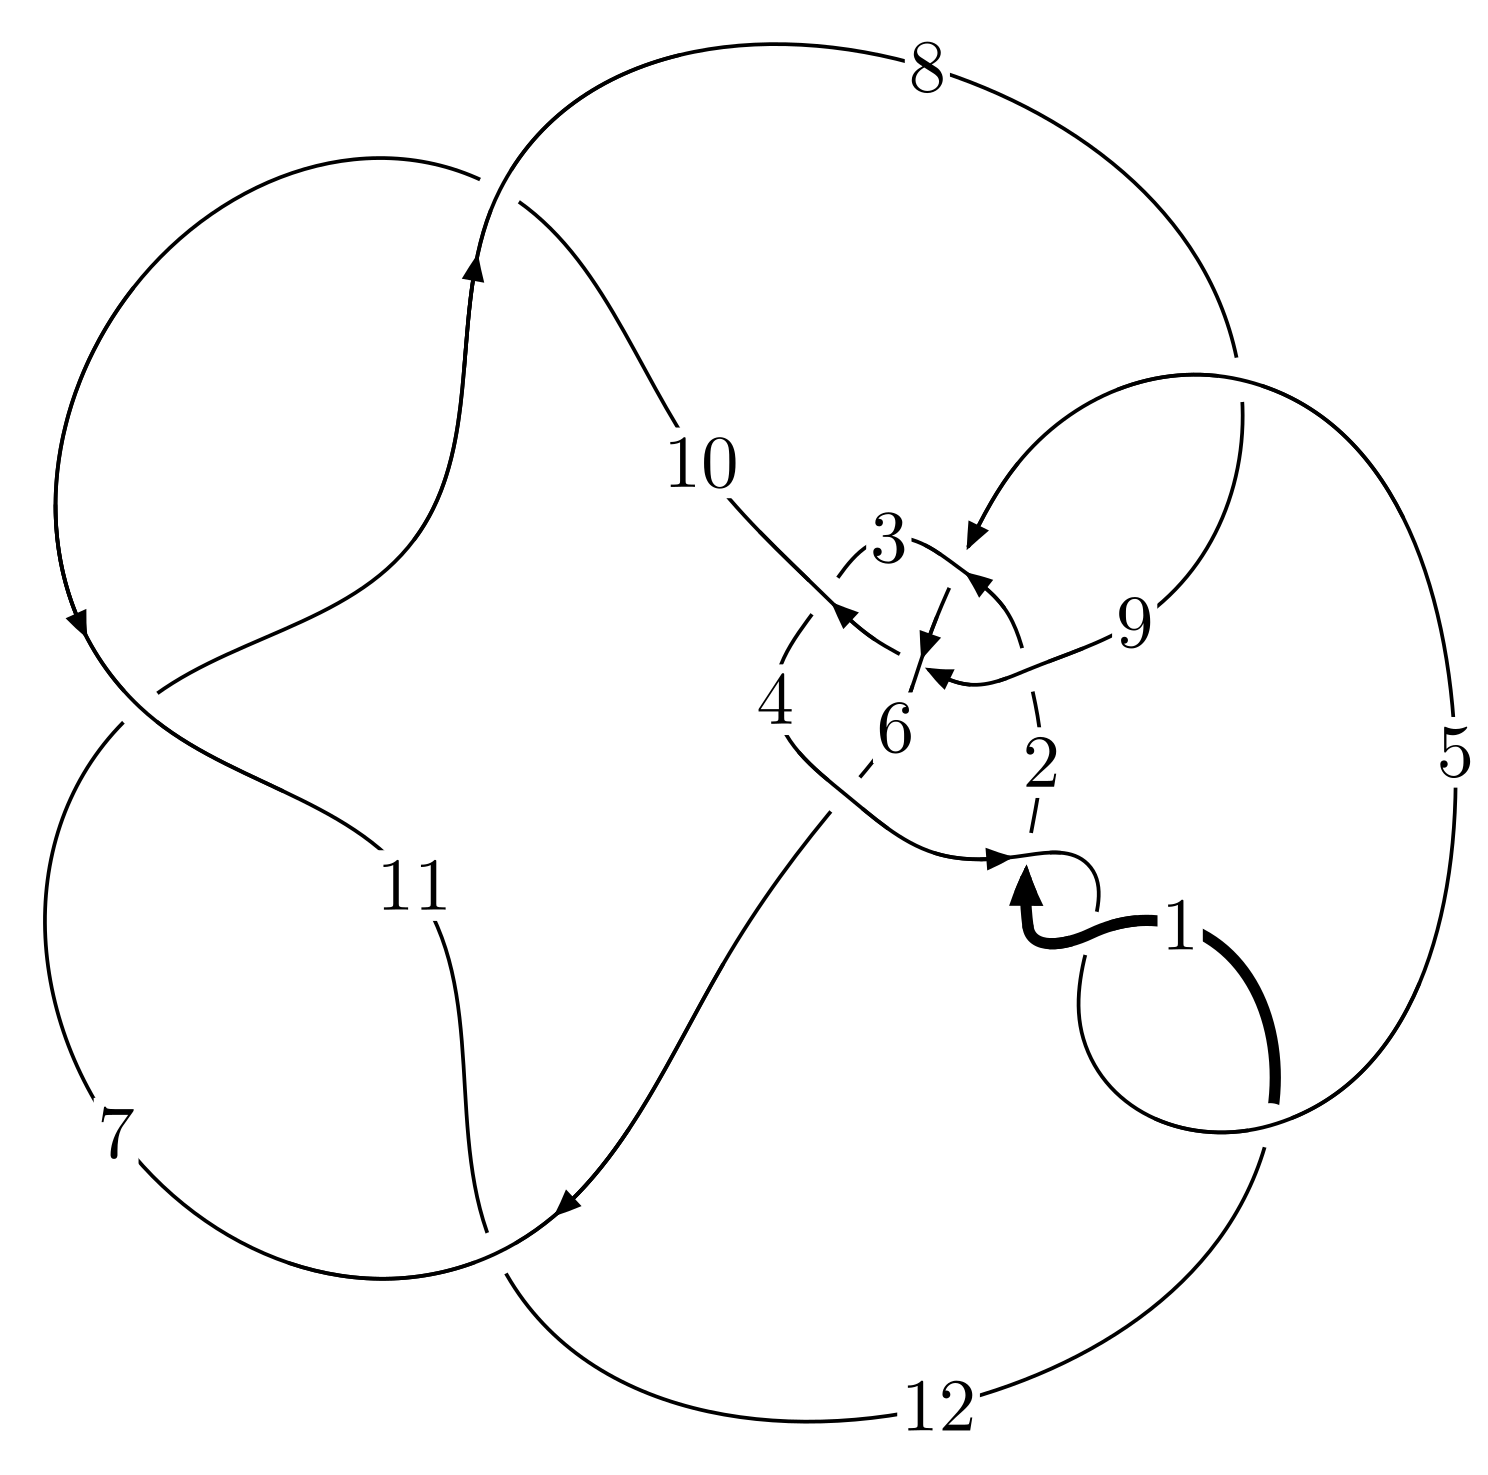
\includegraphics[width=112pt]{../../../GIT/diagram.site/Diagrams/png/2822_12n_0733.png}\\
\ \ \ A knot diagram\footnotemark}&
\allowdisplaybreaks
\textbf{Linearized knot diagam} \\
\cline{2-2}
 &
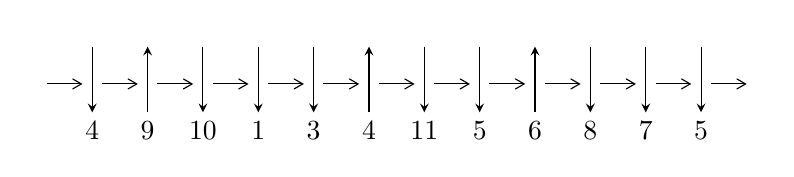
\begin{tikzpicture}[x=20pt, y=17pt]
	% nodes
	\node (C0) at (0, 0) {};
	\node (C1) at (1, 0) {};
	\node (C1U) at (1, +1) {};
	\node (C1D) at (1, -1) {4};

	\node (C2) at (2, 0) {};
	\node (C2U) at (2, +1) {};
	\node (C2D) at (2, -1) {9};

	\node (C3) at (3, 0) {};
	\node (C3U) at (3, +1) {};
	\node (C3D) at (3, -1) {10};

	\node (C4) at (4, 0) {};
	\node (C4U) at (4, +1) {};
	\node (C4D) at (4, -1) {1};

	\node (C5) at (5, 0) {};
	\node (C5U) at (5, +1) {};
	\node (C5D) at (5, -1) {3};

	\node (C6) at (6, 0) {};
	\node (C6U) at (6, +1) {};
	\node (C6D) at (6, -1) {4};

	\node (C7) at (7, 0) {};
	\node (C7U) at (7, +1) {};
	\node (C7D) at (7, -1) {11};

	\node (C8) at (8, 0) {};
	\node (C8U) at (8, +1) {};
	\node (C8D) at (8, -1) {5};

	\node (C9) at (9, 0) {};
	\node (C9U) at (9, +1) {};
	\node (C9D) at (9, -1) {6};

	\node (C10) at (10, 0) {};
	\node (C10U) at (10, +1) {};
	\node (C10D) at (10, -1) {8};

	\node (C11) at (11, 0) {};
	\node (C11U) at (11, +1) {};
	\node (C11D) at (11, -1) {7};

	\node (C12) at (12, 0) {};
	\node (C12U) at (12, +1) {};
	\node (C12D) at (12, -1) {5};
	\node (C13) at (13, 0) {};

	% arrows
	\draw[->,>={angle 60}]
	(C0) edge (C1) (C1) edge (C2) (C2) edge (C3) (C3) edge (C4) (C4) edge (C5) (C5) edge (C6) (C6) edge (C7) (C7) edge (C8) (C8) edge (C9) (C9) edge (C10) (C10) edge (C11) (C11) edge (C12) (C12) edge (C13) ;	\draw[->,>=stealth]
	(C1U) edge (C1D) (C2D) edge (C2U) (C3U) edge (C3D) (C4U) edge (C4D) (C5U) edge (C5D) (C6D) edge (C6U) (C7U) edge (C7D) (C8U) edge (C8D) (C9D) edge (C9U) (C10U) edge (C10D) (C11U) edge (C11D) (C12U) edge (C12D) ;
	\end{tikzpicture} \\
\hhline{~~} \\& 
\textbf{Solving Sequence} \\ \cline{2-2} 
 &
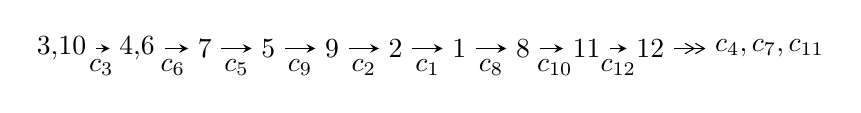
\begin{tikzpicture}[x=23pt, y=7pt]
	% node
	\node (A0) at (-1/8, 0) {3,10};
	\node (A1) at (17/16, 0) {4,6};
	\node (A2) at (17/8, 0) {7};
	\node (A3) at (25/8, 0) {5};
	\node (A4) at (33/8, 0) {9};
	\node (A5) at (41/8, 0) {2};
	\node (A6) at (49/8, 0) {1};
	\node (A7) at (57/8, 0) {8};
	\node (A8) at (65/8, 0) {11};
	\node (A9) at (73/8, 0) {12};
	\node (C1) at (1/2, -1) {$c_{3}$};
	\node (C2) at (13/8, -1) {$c_{6}$};
	\node (C3) at (21/8, -1) {$c_{5}$};
	\node (C4) at (29/8, -1) {$c_{9}$};
	\node (C5) at (37/8, -1) {$c_{2}$};
	\node (C6) at (45/8, -1) {$c_{1}$};
	\node (C7) at (53/8, -1) {$c_{8}$};
	\node (C8) at (61/8, -1) {$c_{10}$};
	\node (C9) at (69/8, -1) {$c_{12}$};
	\node (A10) at (11, 0) {$c_{4},c_{7},c_{11}$};

	% edge
	\draw[->,>=stealth]	
	(A0) edge (A1) (A1) edge (A2) (A2) edge (A3) (A3) edge (A4) (A4) edge (A5) (A5) edge (A6) (A6) edge (A7) (A7) edge (A8) (A8) edge (A9) ;
	\draw[->>,>={angle 60}]	
	(A9) edge (A10);
\end{tikzpicture} \\ 

\end{tabular} \\

\footnotetext{
The image of knot diagram is generated by the software ``\textbf{Draw programme}" developed by Andrew Bartholomew(\url{http://www.layer8.co.uk/maths/draw/index.htm\#Running-draw}), where we modified some parts for our purpose(\url{https://github.com/CATsTAILs/LinksPainter}).
}\phantom \\ \newline 
\centering \textbf{Ideals for irreducible components\footnotemark of $X_{\text{par}}$} 
 
\begin{align*}
I^u_{1}&=\langle 
7.85180\times10^{324} u^{84}-5.53960\times10^{324} u^{83}+\cdots+5.09556\times10^{323} b+5.72110\times10^{326},\\
\phantom{I^u_{1}}&\phantom{= \langle  }5.13372\times10^{326} u^{84}-3.22757\times10^{326} u^{83}+\cdots+1.17198\times10^{325} a+3.19118\times10^{328},\\
\phantom{I^u_{1}}&\phantom{= \langle  }u^{85}- u^{84}+\cdots+171 u-23\rangle \\
I^u_{2}&=\langle 
5 u^{19}-6 u^{18}+\cdots+2 b-13,\;4 u^{19}-5 u^{18}+\cdots+2 a-3,\;u^{20}+3 u^{18}+\cdots+5 u^2+1\rangle \\
\\
\end{align*}
\raggedright * 2 irreducible components of $\dim_{\mathbb{C}}=0$, with total 105 representations.\\
\footnotetext{All coefficients of polynomials are rational numbers. But the coefficients are sometimes approximated in decimal forms when there is not enough margin.}
\newpage
\renewcommand{\arraystretch}{1}
\centering \section*{I. $I^u_{1}= \langle 7.85\times10^{324} u^{84}-5.54\times10^{324} u^{83}+\cdots+5.10\times10^{323} b+5.72\times10^{326},\;5.13\times10^{326} u^{84}-3.23\times10^{326} u^{83}+\cdots+1.17\times10^{325} a+3.19\times10^{328},\;u^{85}- u^{84}+\cdots+171 u-23 \rangle$}
\flushleft \textbf{(i) Arc colorings}\\
\begin{tabular}{m{7pt} m{180pt} m{7pt} m{180pt} }
\flushright $a_{3}=$&$\begin{pmatrix}1\\0\end{pmatrix}$ \\
\flushright $a_{10}=$&$\begin{pmatrix}0\\u\end{pmatrix}$ \\
\flushright $a_{4}=$&$\begin{pmatrix}1\\u^2\end{pmatrix}$ \\
\flushright $a_{6}=$&$\begin{pmatrix}-43.8039 u^{84}+27.5395 u^{83}+\cdots+13107.8 u-2722.90\\-15.4091 u^{84}+10.8714 u^{83}+\cdots+5055.34 u-1122.76\end{pmatrix}$ \\
\flushright $a_{7}=$&$\begin{pmatrix}-53.6006 u^{84}+34.8765 u^{83}+\cdots+16389.4 u-3471.58\\-15.7706 u^{84}+11.3455 u^{83}+\cdots+5250.63 u-1179.34\end{pmatrix}$ \\
\flushright $a_{5}=$&$\begin{pmatrix}-59.2130 u^{84}+38.4110 u^{83}+\cdots+18163.1 u-3845.66\\-15.4091 u^{84}+10.8714 u^{83}+\cdots+5055.34 u-1122.76\end{pmatrix}$ \\
\flushright $a_{9}=$&$\begin{pmatrix}-100.072 u^{84}+57.1100 u^{83}+\cdots+27587.5 u-5300.30\\-27.6763 u^{84}+16.6280 u^{83}+\cdots+7904.83 u-1574.20\end{pmatrix}$ \\
\flushright $a_{2}=$&$\begin{pmatrix}-32.2653 u^{84}+25.7906 u^{83}+\cdots+11118.1 u-2655.82\\17.9359 u^{84}-11.0484 u^{83}+\cdots-5175.15 u+1047.54\end{pmatrix}$ \\
\flushright $a_{1}=$&$\begin{pmatrix}-14.0239 u^{84}+13.3991 u^{83}+\cdots+5577.88 u-1459.36\\19.8199 u^{84}-12.5011 u^{83}+\cdots-5755.92 u+1182.08\end{pmatrix}$ \\
\flushright $a_{8}=$&$\begin{pmatrix}-63.1948 u^{84}+34.9424 u^{83}+\cdots+17087.5 u-3198.98\\-17.6497 u^{84}+7.33319 u^{83}+\cdots+4042.64 u-585.929\end{pmatrix}$ \\
\flushright $a_{11}=$&$\begin{pmatrix}23.0154 u^{84}-12.3805 u^{83}+\cdots-5914.82 u+1084.83\\-55.2963 u^{84}+33.1820 u^{83}+\cdots+15690.5 u-3105.92\end{pmatrix}$ \\
\flushright $a_{12}=$&$\begin{pmatrix}-59.0148 u^{84}+37.4295 u^{83}+\cdots+17255.2 u-3578.54\\43.6488 u^{84}-27.5891 u^{83}+\cdots-12864.2 u+2648.65\end{pmatrix}$\\&\end{tabular}
\flushleft \textbf{(ii) Obstruction class $= -1$}\\~\\
\flushleft \textbf{(iii) Cusp Shapes $= 31.3947 u^{84}-16.5057 u^{83}+\cdots-10580.4 u+2033.20$}\\~\\
\newpage\renewcommand{\arraystretch}{1}
\flushleft \textbf{(iv) u-Polynomials at the component}\newline \\
\begin{tabular}{m{50pt}|m{274pt}}
Crossings & \hspace{64pt}u-Polynomials at each crossing \\
\hline $$\begin{aligned}c_{1},c_{4},c_{12}\end{aligned}$$&$\begin{aligned}
&u^{85}+5 u^{84}+\cdots+97 u+11
\end{aligned}$\\
\hline $$\begin{aligned}c_{2}\end{aligned}$$&$\begin{aligned}
&u^{85}- u^{84}+\cdots+301 u+71
\end{aligned}$\\
\hline $$\begin{aligned}c_{3}\end{aligned}$$&$\begin{aligned}
&u^{85}+u^{84}+\cdots+171 u+23
\end{aligned}$\\
\hline $$\begin{aligned}c_{5}\end{aligned}$$&$\begin{aligned}
&u^{85}-3 u^{84}+\cdots-22 u+3
\end{aligned}$\\
\hline $$\begin{aligned}c_{6}\end{aligned}$$&$\begin{aligned}
&u^{85}-2 u^{84}+\cdots+54441 u+8717
\end{aligned}$\\
\hline $$\begin{aligned}c_{7},c_{10},c_{11}\end{aligned}$$&$\begin{aligned}
&u^{85}+3 u^{84}+\cdots-31 u+21
\end{aligned}$\\
\hline $$\begin{aligned}c_{8}\end{aligned}$$&$\begin{aligned}
&u^{85}-2 u^{84}+\cdots-43138551 u+7230569
\end{aligned}$\\
\hline $$\begin{aligned}c_{9}\end{aligned}$$&$\begin{aligned}
&u^{85}-5 u^{84}+\cdots+9 u+1
\end{aligned}$\\
\hline
\end{tabular}\\~\\
\newpage\renewcommand{\arraystretch}{1}
\flushleft \textbf{(v) Riley Polynomials at the component}\newline \\
\begin{tabular}{m{50pt}|m{274pt}}
Crossings & \hspace{64pt}Riley Polynomials at each crossing \\
\hline $$\begin{aligned}c_{1},c_{4},c_{12}\end{aligned}$$&$\begin{aligned}
&y^{85}+31 y^{84}+\cdots-4605 y-121
\end{aligned}$\\
\hline $$\begin{aligned}c_{2}\end{aligned}$$&$\begin{aligned}
&y^{85}+25 y^{84}+\cdots-1039577 y-5041
\end{aligned}$\\
\hline $$\begin{aligned}c_{3}\end{aligned}$$&$\begin{aligned}
&y^{85}-3 y^{84}+\cdots+25423 y-529
\end{aligned}$\\
\hline $$\begin{aligned}c_{5}\end{aligned}$$&$\begin{aligned}
&y^{85}-5 y^{84}+\cdots+454 y-9
\end{aligned}$\\
\hline $$\begin{aligned}c_{6}\end{aligned}$$&$\begin{aligned}
&y^{85}+32 y^{84}+\cdots-3915581617 y-75986089
\end{aligned}$\\
\hline $$\begin{aligned}c_{7},c_{10},c_{11}\end{aligned}$$&$\begin{aligned}
&y^{85}+73 y^{84}+\cdots+247 y-441
\end{aligned}$\\
\hline $$\begin{aligned}c_{8}\end{aligned}$$&$\begin{aligned}
&y^{85}-24 y^{84}+\cdots+583651994447037 y-52281128063761
\end{aligned}$\\
\hline $$\begin{aligned}c_{9}\end{aligned}$$&$\begin{aligned}
&y^{85}+5 y^{84}+\cdots+13 y-1
\end{aligned}$\\
\hline
\end{tabular}\\~\\
\newpage\flushleft \textbf{(vi) Complex Volumes and Cusp Shapes}
$$\begin{array}{c|c|c}  
\text{Solutions to }I^u_{1}& \I (\text{vol} + \sqrt{-1}CS) & \text{Cusp shape}\\
 \hline 
\begin{aligned}
u &= \phantom{-}0.831046 + 0.557044 I \\
a &= -0.241571 - 0.365025 I \\
b &= \phantom{-}0.849319 + 0.261416 I\end{aligned}
 & -1.44654 - 0.25256 I & \phantom{-0.000000 } 0 \\ \hline\begin{aligned}
u &= \phantom{-}0.831046 - 0.557044 I \\
a &= -0.241571 + 0.365025 I \\
b &= \phantom{-}0.849319 - 0.261416 I\end{aligned}
 & -1.44654 + 0.25256 I & \phantom{-0.000000 } 0 \\ \hline\begin{aligned}
u &= -0.127487 + 0.957078 I \\
a &= \phantom{-}0.638468 - 1.021490 I \\
b &= -0.698591 + 1.035080 I\end{aligned}
 & \phantom{-}6.99156 + 0.55070 I & \phantom{-0.000000 } 0 \\ \hline\begin{aligned}
u &= -0.127487 - 0.957078 I \\
a &= \phantom{-}0.638468 + 1.021490 I \\
b &= -0.698591 - 1.035080 I\end{aligned}
 & \phantom{-}6.99156 - 0.55070 I & \phantom{-0.000000 } 0 \\ \hline\begin{aligned}
u &= -0.813260 + 0.513670 I \\
a &= \phantom{-}0.488792 + 0.961975 I \\
b &= \phantom{-}0.309711 - 0.495129 I\end{aligned}
 & \phantom{-}1.12817 + 2.01460 I & \phantom{-0.000000 } 0 \\ \hline\begin{aligned}
u &= -0.813260 - 0.513670 I \\
a &= \phantom{-}0.488792 - 0.961975 I \\
b &= \phantom{-}0.309711 + 0.495129 I\end{aligned}
 & \phantom{-}1.12817 - 2.01460 I & \phantom{-0.000000 } 0 \\ \hline\begin{aligned}
u &= -0.698511 + 0.631519 I \\
a &= -0.566077 - 1.087700 I \\
b &= -1.27175 + 0.92234 I\end{aligned}
 & \phantom{-}5.16779 + 6.57404 I & \phantom{-0.000000 } 0 \\ \hline\begin{aligned}
u &= -0.698511 - 0.631519 I \\
a &= -0.566077 + 1.087700 I \\
b &= -1.27175 - 0.92234 I\end{aligned}
 & \phantom{-}5.16779 - 6.57404 I & \phantom{-0.000000 } 0 \\ \hline\begin{aligned}
u &= -0.818146 + 0.459472 I \\
a &= \phantom{-}0.31309 + 1.54710 I \\
b &= \phantom{-}0.747796 - 0.917953 I\end{aligned}
 & \phantom{-}0.55790 + 4.56915 I & \phantom{-0.000000 } 0 \\ \hline\begin{aligned}
u &= -0.818146 - 0.459472 I \\
a &= \phantom{-}0.31309 - 1.54710 I \\
b &= \phantom{-}0.747796 + 0.917953 I\end{aligned}
 & \phantom{-}0.55790 - 4.56915 I & \phantom{-0.000000 } 0\\
 \hline 
 \end{array}$$\newpage$$\begin{array}{c|c|c}  
\text{Solutions to }I^u_{1}& \I (\text{vol} + \sqrt{-1}CS) & \text{Cusp shape}\\
 \hline 
\begin{aligned}
u &= \phantom{-}0.065336 + 0.910896 I \\
a &= \phantom{-}1.115130 + 0.555808 I \\
b &= -0.547614 - 0.217318 I\end{aligned}
 & -0.64133 - 2.51721 I & \phantom{-0.000000 } 0 \\ \hline\begin{aligned}
u &= \phantom{-}0.065336 - 0.910896 I \\
a &= \phantom{-}1.115130 - 0.555808 I \\
b &= -0.547614 + 0.217318 I\end{aligned}
 & -0.64133 + 2.51721 I & \phantom{-0.000000 } 0 \\ \hline\begin{aligned}
u &= \phantom{-}0.882759 + 0.165692 I \\
a &= \phantom{-}0.145743 + 1.002340 I \\
b &= \phantom{-}0.85643 - 1.48425 I\end{aligned}
 & \phantom{-}0.54061 + 5.76543 I & \phantom{-0.000000 } 0 \\ \hline\begin{aligned}
u &= \phantom{-}0.882759 - 0.165692 I \\
a &= \phantom{-}0.145743 - 1.002340 I \\
b &= \phantom{-}0.85643 + 1.48425 I\end{aligned}
 & \phantom{-}0.54061 - 5.76543 I & \phantom{-0.000000 } 0 \\ \hline\begin{aligned}
u &= \phantom{-}0.885894\phantom{ +0.000000I} \\
a &= \phantom{-}0.163031\phantom{ +0.000000I} \\
b &= \phantom{-}0.708021\phantom{ +0.000000I}\end{aligned}
 & -1.16186\phantom{ +0.000000I} & \phantom{-0.000000 } 0 \\ \hline\begin{aligned}
u &= \phantom{-}1.034170 + 0.415668 I \\
a &= \phantom{-}0.520931 - 1.110500 I \\
b &= \phantom{-}1.08674 + 1.06190 I\end{aligned}
 & \phantom{-}3.59865 - 4.22466 I & \phantom{-0.000000 } 0 \\ \hline\begin{aligned}
u &= \phantom{-}1.034170 - 0.415668 I \\
a &= \phantom{-}0.520931 + 1.110500 I \\
b &= \phantom{-}1.08674 - 1.06190 I\end{aligned}
 & \phantom{-}3.59865 + 4.22466 I & \phantom{-0.000000 } 0 \\ \hline\begin{aligned}
u &= -0.742150 + 0.452220 I \\
a &= \phantom{-}0.137812 + 0.901496 I \\
b &= -0.35871 - 1.48351 I\end{aligned}
 & \phantom{-}0.464606 + 0.538811 I & \phantom{-0.000000 } 0 \\ \hline\begin{aligned}
u &= -0.742150 - 0.452220 I \\
a &= \phantom{-}0.137812 - 0.901496 I \\
b &= -0.35871 + 1.48351 I\end{aligned}
 & \phantom{-}0.464606 - 0.538811 I & \phantom{-0.000000 } 0 \\ \hline\begin{aligned}
u &= \phantom{-}0.533262 + 0.684484 I \\
a &= -0.49644 - 1.55374 I \\
b &= \phantom{-}0.412791 + 1.193030 I\end{aligned}
 & \phantom{-}5.66071 - 5.76005 I & \phantom{-0.000000 } 0\\
 \hline 
 \end{array}$$\newpage$$\begin{array}{c|c|c}  
\text{Solutions to }I^u_{1}& \I (\text{vol} + \sqrt{-1}CS) & \text{Cusp shape}\\
 \hline 
\begin{aligned}
u &= \phantom{-}0.533262 - 0.684484 I \\
a &= -0.49644 + 1.55374 I \\
b &= \phantom{-}0.412791 - 1.193030 I\end{aligned}
 & \phantom{-}5.66071 + 5.76005 I & \phantom{-0.000000 } 0 \\ \hline\begin{aligned}
u &= -0.857850 + 0.050796 I \\
a &= \phantom{-}1.66393 - 1.08609 I \\
b &= \phantom{-}0.939994 + 0.127390 I\end{aligned}
 & \phantom{-}0.12817 - 6.34062 I & \phantom{-0.000000 } 0 \\ \hline\begin{aligned}
u &= -0.857850 - 0.050796 I \\
a &= \phantom{-}1.66393 + 1.08609 I \\
b &= \phantom{-}0.939994 - 0.127390 I\end{aligned}
 & \phantom{-}0.12817 + 6.34062 I & \phantom{-0.000000 } 0 \\ \hline\begin{aligned}
u &= -0.655503 + 0.529519 I \\
a &= \phantom{-}1.70492 + 0.55646 I \\
b &= \phantom{-}0.482345 - 0.572650 I\end{aligned}
 & \phantom{-}0.80709 + 3.24268 I & \phantom{-0.000000 } 0 \\ \hline\begin{aligned}
u &= -0.655503 - 0.529519 I \\
a &= \phantom{-}1.70492 - 0.55646 I \\
b &= \phantom{-}0.482345 + 0.572650 I\end{aligned}
 & \phantom{-}0.80709 - 3.24268 I & \phantom{-0.000000 } 0 \\ \hline\begin{aligned}
u &= -1.162410 + 0.089791 I \\
a &= -0.106902 - 0.116132 I \\
b &= \phantom{-}0.897619 + 0.731041 I\end{aligned}
 & \phantom{-}3.40154 - 2.94778 I & \phantom{-0.000000 } 0 \\ \hline\begin{aligned}
u &= -1.162410 - 0.089791 I \\
a &= -0.106902 + 0.116132 I \\
b &= \phantom{-}0.897619 - 0.731041 I\end{aligned}
 & \phantom{-}3.40154 + 2.94778 I & \phantom{-0.000000 } 0 \\ \hline\begin{aligned}
u &= \phantom{-}0.439950 + 0.685441 I \\
a &= -0.01004 + 1.48686 I \\
b &= -0.983699 - 0.818536 I\end{aligned}
 & \phantom{-}2.22530 - 3.06319 I & \phantom{-0.000000 } 0 \\ \hline\begin{aligned}
u &= \phantom{-}0.439950 - 0.685441 I \\
a &= -0.01004 - 1.48686 I \\
b &= -0.983699 + 0.818536 I\end{aligned}
 & \phantom{-}2.22530 + 3.06319 I & \phantom{-0.000000 } 0 \\ \hline\begin{aligned}
u &= \phantom{-}0.567035 + 0.546622 I \\
a &= -2.47306 + 0.15550 I \\
b &= -0.473503 - 0.438600 I\end{aligned}
 & \phantom{-}1.97158 - 8.71574 I & -6.0000 + 13.5098 I\\
 \hline 
 \end{array}$$\newpage$$\begin{array}{c|c|c}  
\text{Solutions to }I^u_{1}& \I (\text{vol} + \sqrt{-1}CS) & \text{Cusp shape}\\
 \hline 
\begin{aligned}
u &= \phantom{-}0.567035 - 0.546622 I \\
a &= -2.47306 - 0.15550 I \\
b &= -0.473503 + 0.438600 I\end{aligned}
 & \phantom{-}1.97158 + 8.71574 I & -6.0000 - 13.5098 I \\ \hline\begin{aligned}
u &= \phantom{-}0.913597 + 0.809553 I \\
a &= -0.285654 + 0.490373 I \\
b &= -0.86921 - 1.39950 I\end{aligned}
 & \phantom{-}7.94883 - 3.03290 I & \phantom{-0.000000 } 0 \\ \hline\begin{aligned}
u &= \phantom{-}0.913597 - 0.809553 I \\
a &= -0.285654 - 0.490373 I \\
b &= -0.86921 + 1.39950 I\end{aligned}
 & \phantom{-}7.94883 + 3.03290 I & \phantom{-0.000000 } 0 \\ \hline\begin{aligned}
u &= \phantom{-}0.629450 + 0.446816 I \\
a &= \phantom{-}0.026130 - 0.904408 I \\
b &= -0.99443 + 1.41472 I\end{aligned}
 & -2.93325 - 4.48039 I & -9.85243 + 10.13391 I \\ \hline\begin{aligned}
u &= \phantom{-}0.629450 - 0.446816 I \\
a &= \phantom{-}0.026130 + 0.904408 I \\
b &= -0.99443 - 1.41472 I\end{aligned}
 & -2.93325 + 4.48039 I & -9.85243 - 10.13391 I \\ \hline\begin{aligned}
u &= \phantom{-}0.692510 + 0.288611 I \\
a &= \phantom{-}2.40204 + 0.20862 I \\
b &= \phantom{-}0.646277 + 0.227329 I\end{aligned}
 & -3.31554 + 1.59248 I & -13.85520 + 2.64790 I \\ \hline\begin{aligned}
u &= \phantom{-}0.692510 - 0.288611 I \\
a &= \phantom{-}2.40204 - 0.20862 I \\
b &= \phantom{-}0.646277 - 0.227329 I\end{aligned}
 & -3.31554 - 1.59248 I & -13.85520 - 2.64790 I \\ \hline\begin{aligned}
u &= -0.565001 + 0.454183 I \\
a &= -0.066232 + 0.868689 I \\
b &= -1.48274 - 1.36869 I\end{aligned}
 & \phantom{-}1.49507 + 8.52247 I & -6.0000 - 12.9551 I \\ \hline\begin{aligned}
u &= -0.565001 - 0.454183 I \\
a &= -0.066232 - 0.868689 I \\
b &= -1.48274 + 1.36869 I\end{aligned}
 & \phantom{-}1.49507 - 8.52247 I & -6.0000 + 12.9551 I \\ \hline\begin{aligned}
u &= -0.709761 + 0.020702 I \\
a &= \phantom{-}0.646694 - 1.140950 I \\
b &= -0.334689 + 0.046125 I\end{aligned}
 & \phantom{-}0.51104 - 2.01003 I & -2.20570 + 3.99950 I\\
 \hline 
 \end{array}$$\newpage$$\begin{array}{c|c|c}  
\text{Solutions to }I^u_{1}& \I (\text{vol} + \sqrt{-1}CS) & \text{Cusp shape}\\
 \hline 
\begin{aligned}
u &= -0.709761 - 0.020702 I \\
a &= \phantom{-}0.646694 + 1.140950 I \\
b &= -0.334689 - 0.046125 I\end{aligned}
 & \phantom{-}0.51104 + 2.01003 I & -2.20570 - 3.99950 I \\ \hline\begin{aligned}
u &= \phantom{-}1.292070 + 0.003692 I \\
a &= \phantom{-}0.408255 + 0.744650 I \\
b &= \phantom{-}0.251664 + 0.213807 I\end{aligned}
 & \phantom{-}2.52430 + 1.99992 I & \phantom{-0.000000 } 0 \\ \hline\begin{aligned}
u &= \phantom{-}1.292070 - 0.003692 I \\
a &= \phantom{-}0.408255 - 0.744650 I \\
b &= \phantom{-}0.251664 - 0.213807 I\end{aligned}
 & \phantom{-}2.52430 - 1.99992 I & \phantom{-0.000000 } 0 \\ \hline\begin{aligned}
u &= \phantom{-}0.925904 + 0.944482 I \\
a &= \phantom{-}0.215413 - 1.215970 I \\
b &= \phantom{-}0.270846 + 0.684713 I\end{aligned}
 & \phantom{-}8.96391 - 3.46153 I & \phantom{-0.000000 } 0 \\ \hline\begin{aligned}
u &= \phantom{-}0.925904 - 0.944482 I \\
a &= \phantom{-}0.215413 + 1.215970 I \\
b &= \phantom{-}0.270846 - 0.684713 I\end{aligned}
 & \phantom{-}8.96391 + 3.46153 I & \phantom{-0.000000 } 0 \\ \hline\begin{aligned}
u &= -0.670949 + 0.083829 I \\
a &= \phantom{-}0.109150 - 1.101600 I \\
b &= \phantom{-}1.19113 + 1.28717 I\end{aligned}
 & -4.30679 - 2.27536 I & -16.5563 + 2.4540 I \\ \hline\begin{aligned}
u &= -0.670949 - 0.083829 I \\
a &= \phantom{-}0.109150 + 1.101600 I \\
b &= \phantom{-}1.19113 - 1.28717 I\end{aligned}
 & -4.30679 + 2.27536 I & -16.5563 - 2.4540 I \\ \hline\begin{aligned}
u &= -0.839735 + 1.028720 I \\
a &= -0.024893 - 0.614603 I \\
b &= -0.920321 + 1.054900 I\end{aligned}
 & \phantom{-}3.83581 + 3.87716 I & \phantom{-0.000000 } 0 \\ \hline\begin{aligned}
u &= -0.839735 - 1.028720 I \\
a &= -0.024893 + 0.614603 I \\
b &= -0.920321 - 1.054900 I\end{aligned}
 & \phantom{-}3.83581 - 3.87716 I & \phantom{-0.000000 } 0 \\ \hline\begin{aligned}
u &= \phantom{-}0.612225 + 1.199640 I \\
a &= -0.434189 - 0.108543 I \\
b &= \phantom{-}1.008350 - 0.099538 I\end{aligned}
 & -1.126070 - 0.317400 I & \phantom{-0.000000 } 0\\
 \hline 
 \end{array}$$\newpage$$\begin{array}{c|c|c}  
\text{Solutions to }I^u_{1}& \I (\text{vol} + \sqrt{-1}CS) & \text{Cusp shape}\\
 \hline 
\begin{aligned}
u &= \phantom{-}0.612225 - 1.199640 I \\
a &= -0.434189 + 0.108543 I \\
b &= \phantom{-}1.008350 + 0.099538 I\end{aligned}
 & -1.126070 + 0.317400 I & \phantom{-0.000000 } 0 \\ \hline\begin{aligned}
u &= -0.863786 + 1.085850 I \\
a &= \phantom{-}0.586086 - 0.198313 I \\
b &= -0.428910 - 0.311916 I\end{aligned}
 & -0.35681 - 2.79976 I & \phantom{-0.000000 } 0 \\ \hline\begin{aligned}
u &= -0.863786 - 1.085850 I \\
a &= \phantom{-}0.586086 + 0.198313 I \\
b &= -0.428910 + 0.311916 I\end{aligned}
 & -0.35681 + 2.79976 I & \phantom{-0.000000 } 0 \\ \hline\begin{aligned}
u &= -0.503079 + 0.267304 I \\
a &= -3.34209 + 1.22768 I \\
b &= -0.549342 + 0.188748 I\end{aligned}
 & -3.54083 + 3.55162 I & -16.4796 - 10.7233 I \\ \hline\begin{aligned}
u &= -0.503079 - 0.267304 I \\
a &= -3.34209 - 1.22768 I \\
b &= -0.549342 - 0.188748 I\end{aligned}
 & -3.54083 - 3.55162 I & -16.4796 + 10.7233 I \\ \hline\begin{aligned}
u &= \phantom{-}1.06471 + 0.98078 I \\
a &= \phantom{-}0.010866 + 1.078640 I \\
b &= -1.018890 - 0.794064 I\end{aligned}
 & -1.50860 - 6.81305 I & \phantom{-0.000000 } 0 \\ \hline\begin{aligned}
u &= \phantom{-}1.06471 - 0.98078 I \\
a &= \phantom{-}0.010866 - 1.078640 I \\
b &= -1.018890 + 0.794064 I\end{aligned}
 & -1.50860 + 6.81305 I & \phantom{-0.000000 } 0 \\ \hline\begin{aligned}
u &= -1.09605 + 0.97519 I \\
a &= -0.070271 + 0.951473 I \\
b &= \phantom{-}1.15125 - 1.11120 I\end{aligned}
 & -0.95392 + 10.39970 I & \phantom{-0.000000 } 0 \\ \hline\begin{aligned}
u &= -1.09605 - 0.97519 I \\
a &= -0.070271 - 0.951473 I \\
b &= \phantom{-}1.15125 + 1.11120 I\end{aligned}
 & -0.95392 - 10.39970 I & \phantom{-0.000000 } 0 \\ \hline\begin{aligned}
u &= -1.23789 + 0.80342 I \\
a &= \phantom{-}0.066354 + 0.929504 I \\
b &= \phantom{-}1.041570 - 0.765298 I\end{aligned}
 & -1.47341 + 1.29795 I & \phantom{-0.000000 } 0\\
 \hline 
 \end{array}$$\newpage$$\begin{array}{c|c|c}  
\text{Solutions to }I^u_{1}& \I (\text{vol} + \sqrt{-1}CS) & \text{Cusp shape}\\
 \hline 
\begin{aligned}
u &= -1.23789 - 0.80342 I \\
a &= \phantom{-}0.066354 - 0.929504 I \\
b &= \phantom{-}1.041570 + 0.765298 I\end{aligned}
 & -1.47341 - 1.29795 I & \phantom{-0.000000 } 0 \\ \hline\begin{aligned}
u &= \phantom{-}1.16995 + 0.90072 I \\
a &= -0.006807 - 0.942814 I \\
b &= \phantom{-}1.12371 + 0.95306 I\end{aligned}
 & -5.16019 - 5.88389 I & \phantom{-0.000000 } 0 \\ \hline\begin{aligned}
u &= \phantom{-}1.16995 - 0.90072 I \\
a &= -0.006807 + 0.942814 I \\
b &= \phantom{-}1.12371 - 0.95306 I\end{aligned}
 & -5.16019 + 5.88389 I & \phantom{-0.000000 } 0 \\ \hline\begin{aligned}
u &= \phantom{-}0.70125 + 1.31396 I \\
a &= \phantom{-}0.209393 + 0.604652 I \\
b &= -1.06478 - 1.01972 I\end{aligned}
 & \phantom{-}7.55142 - 5.35757 I & \phantom{-0.000000 } 0 \\ \hline\begin{aligned}
u &= \phantom{-}0.70125 - 1.31396 I \\
a &= \phantom{-}0.209393 - 0.604652 I \\
b &= -1.06478 + 1.01972 I\end{aligned}
 & \phantom{-}7.55142 + 5.35757 I & \phantom{-0.000000 } 0 \\ \hline\begin{aligned}
u &= -1.18191 + 0.99684 I \\
a &= -0.037548 - 1.016460 I \\
b &= -1.12549 + 0.95882 I\end{aligned}
 & -3.93658 + 12.48330 I & \phantom{-0.000000 } 0 \\ \hline\begin{aligned}
u &= -1.18191 - 0.99684 I \\
a &= -0.037548 + 1.016460 I \\
b &= -1.12549 - 0.95882 I\end{aligned}
 & -3.93658 - 12.48330 I & \phantom{-0.000000 } 0 \\ \hline\begin{aligned}
u &= -0.80028 + 1.33460 I \\
a &= \phantom{-}0.188249 - 0.910710 I \\
b &= -0.583389 + 0.702703 I\end{aligned}
 & \phantom{-}8.95846 + 5.01025 I & \phantom{-0.000000 } 0 \\ \hline\begin{aligned}
u &= -0.80028 - 1.33460 I \\
a &= \phantom{-}0.188249 + 0.910710 I \\
b &= -0.583389 - 0.702703 I\end{aligned}
 & \phantom{-}8.95846 - 5.01025 I & \phantom{-0.000000 } 0 \\ \hline\begin{aligned}
u &= \phantom{-}0.298583 + 0.277764 I \\
a &= -1.20840 - 1.79229 I \\
b &= -1.026940 - 0.385412 I\end{aligned}
 & \phantom{-}6.40230 - 2.27863 I & -0.89056 + 3.31839 I\\
 \hline 
 \end{array}$$\newpage$$\begin{array}{c|c|c}  
\text{Solutions to }I^u_{1}& \I (\text{vol} + \sqrt{-1}CS) & \text{Cusp shape}\\
 \hline 
\begin{aligned}
u &= \phantom{-}0.298583 - 0.277764 I \\
a &= -1.20840 + 1.79229 I \\
b &= -1.026940 + 0.385412 I\end{aligned}
 & \phantom{-}6.40230 + 2.27863 I & -0.89056 - 3.31839 I \\ \hline\begin{aligned}
u &= \phantom{-}0.398620 + 0.060755 I \\
a &= \phantom{-}0.13074 + 1.54798 I \\
b &= \phantom{-}1.74001 - 1.00437 I\end{aligned}
 & -1.25022 - 1.15331 I & -15.9982 + 3.4831 I \\ \hline\begin{aligned}
u &= \phantom{-}0.398620 - 0.060755 I \\
a &= \phantom{-}0.13074 - 1.54798 I \\
b &= \phantom{-}1.74001 + 1.00437 I\end{aligned}
 & -1.25022 + 1.15331 I & -15.9982 - 3.4831 I \\ \hline\begin{aligned}
u &= \phantom{-}0.398550 + 0.050882 I \\
a &= -2.05034 + 3.97773 I \\
b &= -0.672123 - 0.119936 I\end{aligned}
 & -1.36735 - 2.11678 I & -15.1062 + 0.7883 I \\ \hline\begin{aligned}
u &= \phantom{-}0.398550 - 0.050882 I \\
a &= -2.05034 - 3.97773 I \\
b &= -0.672123 + 0.119936 I\end{aligned}
 & -1.36735 + 2.11678 I & -15.1062 - 0.7883 I \\ \hline\begin{aligned}
u &= \phantom{-}1.23465 + 1.03140 I \\
a &= -0.040428 + 0.975733 I \\
b &= -1.14414 - 1.10028 I\end{aligned}
 & \phantom{-}1.3879 - 17.4955 I & \phantom{-0.000000 } 0 \\ \hline\begin{aligned}
u &= \phantom{-}1.23465 - 1.03140 I \\
a &= -0.040428 - 0.975733 I \\
b &= -1.14414 + 1.10028 I\end{aligned}
 & \phantom{-}1.3879 + 17.4955 I & \phantom{-0.000000 } 0 \\ \hline\begin{aligned}
u &= -1.16076 + 1.57900 I \\
a &= -0.296277 - 0.026335 I \\
b &= \phantom{-}0.553572 + 0.338879 I\end{aligned}
 & -2.86751 - 3.88898 I & \phantom{-0.000000 } 0 \\ \hline\begin{aligned}
u &= -1.16076 - 1.57900 I \\
a &= -0.296277 + 0.026335 I \\
b &= \phantom{-}0.553572 - 0.338879 I\end{aligned}
 & -2.86751 + 3.88898 I & \phantom{-0.000000 } 0 \\ \hline\begin{aligned}
u &= \phantom{-}1.16470 + 1.57762 I \\
a &= \phantom{-}0.304904 + 0.157476 I \\
b &= -0.541884 + 0.107530 I\end{aligned}
 & -3.58768 - 2.35741 I & \phantom{-0.000000 } 0\\
 \hline 
 \end{array}$$\newpage$$\begin{array}{c|c|c}  
\text{Solutions to }I^u_{1}& \I (\text{vol} + \sqrt{-1}CS) & \text{Cusp shape}\\
 \hline 
\begin{aligned}
u &= \phantom{-}1.16470 - 1.57762 I \\
a &= \phantom{-}0.304904 - 0.157476 I \\
b &= -0.541884 - 0.107530 I\end{aligned}
 & -3.58768 + 2.35741 I & \phantom{-0.000000 } 0 \\ \hline\begin{aligned}
u &= -1.33827 + 1.50559 I \\
a &= \phantom{-}0.216380 - 0.253403 I \\
b &= -0.719339 + 0.135725 I\end{aligned}
 & \phantom{-}0.67050 + 7.44603 I & \phantom{-0.000000 } 0 \\ \hline\begin{aligned}
u &= -1.33827 - 1.50559 I \\
a &= \phantom{-}0.216380 + 0.253403 I \\
b &= -0.719339 - 0.135725 I\end{aligned}
 & \phantom{-}0.67050 - 7.44603 I & \phantom{-0.000000 } 0 \\ \hline\begin{aligned}
u &= \phantom{-}1.04952 + 1.76023 I \\
a &= -0.334642 + 0.135942 I \\
b &= \phantom{-}0.395360 - 0.575779 I\end{aligned}
 & \phantom{-}2.69608 + 8.47155 I & \phantom{-0.000000 } 0 \\ \hline\begin{aligned}
u &= \phantom{-}1.04952 - 1.76023 I \\
a &= -0.334642 - 0.135942 I \\
b &= \phantom{-}0.395360 + 0.575779 I\end{aligned}
 & \phantom{-}2.69608 - 8.47155 I & \phantom{-0.000000 } 0\\
 \hline 
 \end{array}$$\newpage\newpage\renewcommand{\arraystretch}{1}
\centering \section*{II. $I^u_{2}= \langle 5 u^{19}-6 u^{18}+\cdots+2 b-13,\;4 u^{19}-5 u^{18}+\cdots+2 a-3,\;u^{20}+3 u^{18}+\cdots+5 u^2+1 \rangle$}
\flushleft \textbf{(i) Arc colorings}\\
\begin{tabular}{m{7pt} m{180pt} m{7pt} m{180pt} }
\flushright $a_{3}=$&$\begin{pmatrix}1\\0\end{pmatrix}$ \\
\flushright $a_{10}=$&$\begin{pmatrix}0\\u\end{pmatrix}$ \\
\flushright $a_{4}=$&$\begin{pmatrix}1\\u^2\end{pmatrix}$ \\
\flushright $a_{6}=$&$\begin{pmatrix}-2 u^{19}+\frac{5}{2} u^{18}+\cdots-\frac{7}{2} u+\frac{3}{2}\\-\frac{5}{2} u^{19}+3 u^{18}+\cdots-4 u+\frac{13}{2}\end{pmatrix}$ \\
\flushright $a_{7}=$&$\begin{pmatrix}-5 u^{19}+\frac{15}{2} u^{18}+\cdots-\frac{19}{2} u+\frac{21}{2}\\-\frac{3}{2} u^{19}-3 u^{17}+\cdots- u+\frac{3}{2}\end{pmatrix}$ \\
\flushright $a_{5}=$&$\begin{pmatrix}-\frac{9}{2} u^{19}+\frac{11}{2} u^{18}+\cdots-\frac{15}{2} u+8\\-\frac{5}{2} u^{19}+3 u^{18}+\cdots-4 u+\frac{13}{2}\end{pmatrix}$ \\
\flushright $a_{9}=$&$\begin{pmatrix}\frac{3}{2} u^{19}+2 u^{18}+\cdots-2 u+\frac{7}{2}\\u^{19}+3 u^{17}+\cdots- u^2+5 u\end{pmatrix}$ \\
\flushright $a_{2}=$&$\begin{pmatrix}\frac{7}{2} u^{19}-\frac{3}{2} u^{18}+\cdots+\frac{7}{2} u+3\\- u^{18}-3 u^{16}+\cdots+u-5\end{pmatrix}$ \\
\flushright $a_{1}=$&$\begin{pmatrix}\frac{11}{2} u^{19}-5 u^{18}+\cdots+8 u-\frac{7}{2}\\-\frac{1}{2} u^{19}+u^{18}+\cdots- u-\frac{3}{2}\end{pmatrix}$ \\
\flushright $a_{8}=$&$\begin{pmatrix}\frac{11}{2} u^{19}+\frac{3}{2} u^{18}+\cdots+\frac{11}{2} u^2+\frac{13}{2} u\\\frac{21}{2} u^{19}+\frac{3}{2} u^{18}+\cdots+\frac{45}{2} u+1\end{pmatrix}$ \\
\flushright $a_{11}=$&$\begin{pmatrix}-\frac{7}{2} u^{19}-\frac{13}{2} u^{18}+\cdots-\frac{11}{2} u-9\\3 u^{19}-\frac{13}{2} u^{18}+\cdots+\frac{5}{2} u-\frac{29}{2}\end{pmatrix}$ \\
\flushright $a_{12}=$&$\begin{pmatrix}\frac{19}{2} u^{19}-\frac{21}{2} u^{18}+\cdots+\frac{27}{2} u-13\\\frac{7}{2} u^{19}-\frac{9}{2} u^{18}+\cdots+\frac{9}{2} u-12\end{pmatrix}$\\&\end{tabular}
\flushleft \textbf{(ii) Obstruction class $= 1$}\\~\\
\flushleft \textbf{(iii) Cusp Shapes $= -36 u^{19}-\frac{3}{2} u^{18}-\frac{181}{2} u^{17}+\frac{55}{2} u^{16}-\frac{555}{2} u^{15}+\frac{143}{2} u^{14}-\frac{641}{2} u^{13}+\frac{261}{2} u^{12}-356 u^{11}+244 u^{10}-252 u^9+\frac{515}{2} u^8-\frac{217}{2} u^7+195 u^6-\frac{377}{2} u^5+\frac{109}{2} u^4-\frac{407}{2} u^3-\frac{51}{2} u^2-\frac{133}{2} u-\frac{29}{2}$}\\~\\
\newpage\renewcommand{\arraystretch}{1}
\flushleft \textbf{(iv) u-Polynomials at the component}\newline \\
\begin{tabular}{m{50pt}|m{274pt}}
Crossings & \hspace{64pt}u-Polynomials at each crossing \\
\hline $$\begin{aligned}c_{1},c_{12}\end{aligned}$$&$\begin{aligned}
&u^{20}-6 u^{19}+\cdots-4 u+1
\end{aligned}$\\
\hline $$\begin{aligned}c_{2}\end{aligned}$$&$\begin{aligned}
&u^{20}+5 u^{18}+\cdots+3 u^2+1
\end{aligned}$\\
\hline $$\begin{aligned}c_{3}\end{aligned}$$&$\begin{aligned}
&u^{20}+3 u^{18}+\cdots+5 u^2+1
\end{aligned}$\\
\hline $$\begin{aligned}c_{4}\end{aligned}$$&$\begin{aligned}
&u^{20}+6 u^{19}+\cdots+4 u+1
\end{aligned}$\\
\hline $$\begin{aligned}c_{5}\end{aligned}$$&$\begin{aligned}
&u^{20}+2 u^{19}+\cdots+5 u+1
\end{aligned}$\\
\hline $$\begin{aligned}c_{6}\end{aligned}$$&$\begin{aligned}
&u^{20}-3 u^{19}+\cdots-22 u+7
\end{aligned}$\\
\hline $$\begin{aligned}c_{7}\end{aligned}$$&$\begin{aligned}
&u^{20}-4 u^{19}+\cdots-4 u+1
\end{aligned}$\\
\hline $$\begin{aligned}c_{8}\end{aligned}$$&$\begin{aligned}
&u^{20}-3 u^{19}+\cdots-8 u+7
\end{aligned}$\\
\hline $$\begin{aligned}c_{9}\end{aligned}$$&$\begin{aligned}
&u^{20}+2 u^{19}+\cdots+u^3+1
\end{aligned}$\\
\hline $$\begin{aligned}c_{10},c_{11}\end{aligned}$$&$\begin{aligned}
&u^{20}+4 u^{19}+\cdots+4 u+1
\end{aligned}$\\
\hline
\end{tabular}\\~\\
\newpage\renewcommand{\arraystretch}{1}
\flushleft \textbf{(v) Riley Polynomials at the component}\newline \\
\begin{tabular}{m{50pt}|m{274pt}}
Crossings & \hspace{64pt}Riley Polynomials at each crossing \\
\hline $$\begin{aligned}c_{1},c_{4},c_{12}\end{aligned}$$&$\begin{aligned}
&y^{20}+12 y^{19}+\cdots+14 y+1
\end{aligned}$\\
\hline $$\begin{aligned}c_{2}\end{aligned}$$&$\begin{aligned}
&y^{20}+10 y^{19}+\cdots+6 y+1
\end{aligned}$\\
\hline $$\begin{aligned}c_{3}\end{aligned}$$&$\begin{aligned}
&y^{20}+6 y^{19}+\cdots+10 y+1
\end{aligned}$\\
\hline $$\begin{aligned}c_{5}\end{aligned}$$&$\begin{aligned}
&y^{20}+22 y^{18}+\cdots+3 y+1
\end{aligned}$\\
\hline $$\begin{aligned}c_{6}\end{aligned}$$&$\begin{aligned}
&y^{20}+5 y^{19}+\cdots+118 y+49
\end{aligned}$\\
\hline $$\begin{aligned}c_{7},c_{10},c_{11}\end{aligned}$$&$\begin{aligned}
&y^{20}+22 y^{19}+\cdots+30 y+1
\end{aligned}$\\
\hline $$\begin{aligned}c_{8}\end{aligned}$$&$\begin{aligned}
&y^{20}+9 y^{19}+\cdots+188 y+49
\end{aligned}$\\
\hline $$\begin{aligned}c_{9}\end{aligned}$$&$\begin{aligned}
&y^{20}-2 y^{19}+\cdots+2 y^2+1
\end{aligned}$\\
\hline
\end{tabular}\\~\\
\newpage\flushleft \textbf{(vi) Complex Volumes and Cusp Shapes}
$$\begin{array}{c|c|c}  
\text{Solutions to }I^u_{2}& \I (\text{vol} + \sqrt{-1}CS) & \text{Cusp shape}\\
 \hline 
\begin{aligned}
u &= -0.812253 + 0.473538 I \\
a &= \phantom{-}0.40490 + 1.57874 I \\
b &= \phantom{-}0.822438 - 0.775505 I\end{aligned}
 & \phantom{-}0.74373 + 4.05917 I & -2.82511 - 0.92977 I \\ \hline\begin{aligned}
u &= -0.812253 - 0.473538 I \\
a &= \phantom{-}0.40490 - 1.57874 I \\
b &= \phantom{-}0.822438 + 0.775505 I\end{aligned}
 & \phantom{-}0.74373 - 4.05917 I & -2.82511 + 0.92977 I \\ \hline\begin{aligned}
u &= \phantom{-}0.906722 + 0.243640 I \\
a &= \phantom{-}0.641070 - 1.213010 I \\
b &= \phantom{-}1.04129 + 1.08334 I\end{aligned}
 & \phantom{-}3.46371 - 5.35086 I & -2.37266 + 7.93016 I \\ \hline\begin{aligned}
u &= \phantom{-}0.906722 - 0.243640 I \\
a &= \phantom{-}0.641070 + 1.213010 I \\
b &= \phantom{-}1.04129 - 1.08334 I\end{aligned}
 & \phantom{-}3.46371 + 5.35086 I & -2.37266 - 7.93016 I \\ \hline\begin{aligned}
u &= \phantom{-}0.192281 + 0.880278 I \\
a &= -0.396919 + 0.625878 I \\
b &= -0.498840 + 0.507368 I\end{aligned}
 & \phantom{-}1.91537 - 7.45410 I & -2.80666 + 5.14772 I \\ \hline\begin{aligned}
u &= \phantom{-}0.192281 - 0.880278 I \\
a &= -0.396919 - 0.625878 I \\
b &= -0.498840 - 0.507368 I\end{aligned}
 & \phantom{-}1.91537 + 7.45410 I & -2.80666 - 5.14772 I \\ \hline\begin{aligned}
u &= -0.734190 + 0.823682 I \\
a &= -0.029249 - 0.671164 I \\
b &= -1.27215 + 1.29437 I\end{aligned}
 & \phantom{-}7.51988 + 3.71646 I & -0.19673 - 7.05119 I \\ \hline\begin{aligned}
u &= -0.734190 - 0.823682 I \\
a &= -0.029249 + 0.671164 I \\
b &= -1.27215 - 1.29437 I\end{aligned}
 & \phantom{-}7.51988 - 3.71646 I & -0.19673 + 7.05119 I \\ \hline\begin{aligned}
u &= -0.061191 + 0.846410 I \\
a &= -0.594260 - 0.639400 I \\
b &= \phantom{-}0.124196 - 0.469734 I\end{aligned}
 & -2.90766 + 2.92514 I & -7.54786 - 3.63695 I \\ \hline\begin{aligned}
u &= -0.061191 - 0.846410 I \\
a &= -0.594260 + 0.639400 I \\
b &= \phantom{-}0.124196 + 0.469734 I\end{aligned}
 & -2.90766 - 2.92514 I & -7.54786 + 3.63695 I\\
 \hline 
 \end{array}$$\newpage$$\begin{array}{c|c|c}  
\text{Solutions to }I^u_{2}& \I (\text{vol} + \sqrt{-1}CS) & \text{Cusp shape}\\
 \hline 
\begin{aligned}
u &= -0.183312 + 0.749144 I \\
a &= -1.08852 + 1.23211 I \\
b &= \phantom{-}0.551678 - 0.088695 I\end{aligned}
 & -0.74515 + 2.10260 I & -3.47918 + 3.64090 I \\ \hline\begin{aligned}
u &= -0.183312 - 0.749144 I \\
a &= -1.08852 - 1.23211 I \\
b &= \phantom{-}0.551678 + 0.088695 I\end{aligned}
 & -0.74515 - 2.10260 I & -3.47918 - 3.64090 I \\ \hline\begin{aligned}
u &= \phantom{-}0.784188 + 0.983742 I \\
a &= -0.091190 - 1.352150 I \\
b &= \phantom{-}0.410802 + 0.663107 I\end{aligned}
 & \phantom{-}8.70280 - 3.92804 I & -1.94399 + 7.70721 I \\ \hline\begin{aligned}
u &= \phantom{-}0.784188 - 0.983742 I \\
a &= -0.091190 + 1.352150 I \\
b &= \phantom{-}0.410802 - 0.663107 I\end{aligned}
 & \phantom{-}8.70280 + 3.92804 I & -1.94399 - 7.70721 I \\ \hline\begin{aligned}
u &= \phantom{-}0.772112 + 1.011950 I \\
a &= -0.058185 + 0.742783 I \\
b &= -0.884281 - 1.057570 I\end{aligned}
 & \phantom{-}4.21490 - 3.96613 I & \phantom{-}6.63586 + 5.76785 I \\ \hline\begin{aligned}
u &= \phantom{-}0.772112 - 1.011950 I \\
a &= -0.058185 - 0.742783 I \\
b &= -0.884281 + 1.057570 I\end{aligned}
 & \phantom{-}4.21490 + 3.96613 I & \phantom{-}6.63586 - 5.76785 I \\ \hline\begin{aligned}
u &= \phantom{-}0.024765 + 0.703217 I \\
a &= -0.730633 + 0.187577 I \\
b &= \phantom{-}1.256050 + 0.516928 I\end{aligned}
 & -0.662120 + 1.113620 I & -1.35328 - 4.61065 I \\ \hline\begin{aligned}
u &= \phantom{-}0.024765 - 0.703217 I \\
a &= -0.730633 - 0.187577 I \\
b &= \phantom{-}1.256050 - 0.516928 I\end{aligned}
 & -0.662120 - 1.113620 I & -1.35328 + 4.61065 I \\ \hline\begin{aligned}
u &= -0.88912 + 1.26358 I \\
a &= -0.057015 - 0.819735 I \\
b &= -0.551188 + 1.009010 I\end{aligned}
 & \phantom{-}10.65320 + 4.50722 I & \phantom{-}4.88959 - 4.33286 I \\ \hline\begin{aligned}
u &= -0.88912 - 1.26358 I \\
a &= -0.057015 + 0.819735 I \\
b &= -0.551188 - 1.009010 I\end{aligned}
 & \phantom{-}10.65320 - 4.50722 I & \phantom{-}4.88959 + 4.33286 I\\
 \hline 
 \end{array}$$\newpage
\newpage\renewcommand{\arraystretch}{1}
\centering \section*{ III. u-Polynomials}
\begin{tabular}{m{50pt}|m{274pt}}
Crossings & \hspace{64pt}u-Polynomials at each crossing \\
\hline $$\begin{aligned}c_{1},c_{12}\end{aligned}$$&$\begin{aligned}
&(u^{20}-6 u^{19}+\cdots-4 u+1)(u^{85}+5 u^{84}+\cdots+97 u+11)
\end{aligned}$\\
\hline $$\begin{aligned}c_{2}\end{aligned}$$&$\begin{aligned}
&(u^{20}+5 u^{18}+\cdots+3 u^2+1)(u^{85}- u^{84}+\cdots+301 u+71)
\end{aligned}$\\
\hline $$\begin{aligned}c_{3}\end{aligned}$$&$\begin{aligned}
&(u^{20}+3 u^{18}+\cdots+5 u^2+1)(u^{85}+u^{84}+\cdots+171 u+23)
\end{aligned}$\\
\hline $$\begin{aligned}c_{4}\end{aligned}$$&$\begin{aligned}
&(u^{20}+6 u^{19}+\cdots+4 u+1)(u^{85}+5 u^{84}+\cdots+97 u+11)
\end{aligned}$\\
\hline $$\begin{aligned}c_{5}\end{aligned}$$&$\begin{aligned}
&(u^{20}+2 u^{19}+\cdots+5 u+1)(u^{85}-3 u^{84}+\cdots-22 u+3)
\end{aligned}$\\
\hline $$\begin{aligned}c_{6}\end{aligned}$$&$\begin{aligned}
&(u^{20}-3 u^{19}+\cdots-22 u+7)(u^{85}-2 u^{84}+\cdots+54441 u+8717)
\end{aligned}$\\
\hline $$\begin{aligned}c_{7}\end{aligned}$$&$\begin{aligned}
&(u^{20}-4 u^{19}+\cdots-4 u+1)(u^{85}+3 u^{84}+\cdots-31 u+21)
\end{aligned}$\\
\hline $$\begin{aligned}c_{8}\end{aligned}$$&$\begin{aligned}
&(u^{20}-3 u^{19}+\cdots-8 u+7)(u^{85}-2 u^{84}+\cdots-4.31386\times10^{7} u+7230569)
\end{aligned}$\\
\hline $$\begin{aligned}c_{9}\end{aligned}$$&$\begin{aligned}
&(u^{20}+2 u^{19}+\cdots+u^3+1)(u^{85}-5 u^{84}+\cdots+9 u+1)
\end{aligned}$\\
\hline $$\begin{aligned}c_{10},c_{11}\end{aligned}$$&$\begin{aligned}
&(u^{20}+4 u^{19}+\cdots+4 u+1)(u^{85}+3 u^{84}+\cdots-31 u+21)
\end{aligned}$\\
\hline
\end{tabular}\newpage\renewcommand{\arraystretch}{1}
\centering \section*{ IV. Riley Polynomials}
\begin{tabular}{m{50pt}|m{274pt}}
Crossings & \hspace{64pt}Riley Polynomials at each crossing \\
\hline $$\begin{aligned}c_{1},c_{4},c_{12}\end{aligned}$$&$\begin{aligned}
&(y^{20}+12 y^{19}+\cdots+14 y+1)(y^{85}+31 y^{84}+\cdots-4605 y-121)
\end{aligned}$\\
\hline $$\begin{aligned}c_{2}\end{aligned}$$&$\begin{aligned}
&(y^{20}+10 y^{19}+\cdots+6 y+1)(y^{85}+25 y^{84}+\cdots-1039577 y-5041)
\end{aligned}$\\
\hline $$\begin{aligned}c_{3}\end{aligned}$$&$\begin{aligned}
&(y^{20}+6 y^{19}+\cdots+10 y+1)(y^{85}-3 y^{84}+\cdots+25423 y-529)
\end{aligned}$\\
\hline $$\begin{aligned}c_{5}\end{aligned}$$&$\begin{aligned}
&(y^{20}+22 y^{18}+\cdots+3 y+1)(y^{85}-5 y^{84}+\cdots+454 y-9)
\end{aligned}$\\
\hline $$\begin{aligned}c_{6}\end{aligned}$$&$\begin{aligned}
&(y^{20}+5 y^{19}+\cdots+118 y+49)\\
&\cdot(y^{85}+32 y^{84}+\cdots-3915581617 y-75986089)
\end{aligned}$\\
\hline $$\begin{aligned}c_{7},c_{10},c_{11}\end{aligned}$$&$\begin{aligned}
&(y^{20}+22 y^{19}+\cdots+30 y+1)(y^{85}+73 y^{84}+\cdots+247 y-441)
\end{aligned}$\\
\hline $$\begin{aligned}c_{8}\end{aligned}$$&$\begin{aligned}
&(y^{20}+9 y^{19}+\cdots+188 y+49)\\
&\cdot(y^{85}-24 y^{84}+\cdots+583651994447037 y-52281128063761)
\end{aligned}$\\
\hline $$\begin{aligned}c_{9}\end{aligned}$$&$\begin{aligned}
&(y^{20}-2 y^{19}+\cdots+2 y^2+1)(y^{85}+5 y^{84}+\cdots+13 y-1)
\end{aligned}$\\
\hline
\end{tabular}
\vskip 2pc
\end{document}